% !TeX root = RJwrapper.tex
\title{dapper: Data Augmentation for Private Posterior Estimation in R}


\author{by Kevin Eng, Jordan A. Awan, Ruobin Gong, Nianqiao Phyllis Ju, and Vinayak A. Rao}

\maketitle

\abstract{%
This paper serves as a reference and introduction on using the dapper R package. It is an MCMC sampling framework which targets the exact posterior distribution given privitized data. The goal of this package is to provide researchers a tool to perform valid Bayesian inference on data protected by differential privacy. A strength of this framework is the ability to target the exact posterior in settings where the likelihood is too complex to analytically express.
}

\hypertarget{introduction}{%
\section{Introduction}\label{introduction}}

Differential privacy provides a rigorous framework for protecting
confidential information from re-identification attacks by using random
noise to obscure the connection between the individual and data (Dwork et al. 2006).
Its development was spurred on by successful attacks
on anonymized data sets containing sensitive personal information. Prior
to differential privacy, anonymization schemes did not always have sound
theoretical guarantees despite appearing adequate. In one instance,
a privacy research was able use a publicly released medical data set
to deduce William Weld, then Governor of Massachusetts, medical diagnoses and prescriptions.
This changed with the introduction of differential privacy and it has served as the theoretical foundation
for many recent advances in privacy technology. Several recent high profile
examples include Apple (Tang et al. 2017), Google (Erlingsson, Pihur, and Korolova 2014), Microsoft (Ding, Kulkarni, and Yekhanin 2017), and the
U.S. Census Bureau (Abowd 2018).

Many data sets that are a target for deploying differential privacy contain
valuable information that stake holders are still interested in
learning about. However, the noise introduced by differential privacy
changes the calculus of inference. As an example,
we can implement differential privacy for tabular data by directly
adding independent, random error to each cell; the amount and type of which is determined by theory. When we fit a regression model to the noise infused data,
this will correspond to having measurement errors
in the covariates. This, unfortunately, violates the assumptions of most statistical models.
In the presence of such errors, standard estimators can exhibit significant bias and incorrect uncertainty quantification
(Gong 2022) (Karwa, Kifer, and Slavković 2015a) (Wang et al. 2018).
These issues are a serious concern for researchers (Santos-Lozada, Howard, and Verdery 2020) (Kenny et al. 2021) (Winkler et al. 2021).
Therefore, developing privacy-aware statistical workflows is necessary in order
for science and privacy to coexists.

Unfortunately, making the necessary adjustments poses formidable mathematical
challenges (Williams and Mcsherry 2010), even for seemingly simple models like linear regression.
The difficulty lies in the marginal likelihood that results from correctly accounting for the injected
privacy noise. This function is often analytically intractable and as a result,
it is difficult or impossible to apply traditional statistical methods
to derive estimators. In particular, the marginal likelihood can involve a complex
integral where it is not even possible to evaluate the likelihood
at a point. Tackling the problem by approximating the likelihood can be computationally
unfeasible since the integral is also of high dimension.
Few tools are available to researchers to address these issues,
and their absence is a serious barrier to the wider adoption
of differential privacy.

The \texttt{dapper} package provides a tool for conducting
valid statistical inference in the presence of privacy noise.
It implements the Bayesian framework proposed by Ju et al. (2022). This framework describes how to modify
an existing Bayesian model to account for privacy noise and \texttt{dapper}
serves as its user-friendly R interface. It allows the
user to specify a sampler from an existing Bayesian model and
automatically constructing a valid posterior sampler that accounts for the
added privacy noise. Compared to other Bayesian approaches, the \texttt{dapper} framework
is model agnostic and requires no tuning parameters. The algorithmic run time
complexity of dapper is similar to the non-private analysis (section 2). The goal of \texttt{dapper} is to provide
a fast, flexible, and user-friendly way to obtain a valid Bayesian analysis of privatized data.

The rest of this article is organized as follows:
Section 2 covers the necessary background to understand the mathematical notation
and ideas used throughout the paper. Section 3 goes over the main algorithm without
going into mathematical detail; for specifics see (Ju et al. 2022). Section 4 provides
an overview of the dapper package and discusses important implementation details.
Section 5 contains two examples of how one might use the package to analyze the
impact of adding noise for privacy. The first example goes over a typical
odds ratio analysis for a \(2 \times 2\) table and the second example
covers a linear regression model.

\hypertarget{background}{%
\section{Background}\label{background}}

Let \(x = (x_1, \ldots, x_n) \in \mathcal{X}^n\) represent a confidential
database containing \(n\) records. We will assume the
data is generated by some statistical model \(f( x \mid \theta)\). It is often the case
some function of \(\theta\) has relevant meaning to the scientific question at hand. In this setting,
learning characteristics of a population reduces to learning about \(\theta\).

In the Bayesian statistical framework, learning about \(\theta\) is
accomplished by using the data \(x\) to update the
posterior \(p(\theta \mid x) \propto f(x \mid \theta) p(\theta)\).
Here, \(p(\theta)\) is called the prior distribution, and represents
the researcher's belief about \(\theta\) before seeing any data. The
posterior represents uncertainty around \(\theta\) and is formed by using Baye's rule to fuse together the
observed data and the research's prior belief.
One major advantage of the Bayesian method is that, through the prior,
it provides a mechanism for incorporating information not explicitly contained
in the data at hand. This is especially useful in settings where there
is considerable domain knowledge on the value of \(\theta\).

For large data sets, it is common to work with a summary statistic \(s = s(x)\)
that has much smaller dimension than the original data. Doing so can
greatly simplify calculations. In general, there can be information
loss with using summary statistics, but for models with a sufficient
statistic, there is no loss. Curators of large databases
often use summary statistics to publish data since it allows them
to efficiently communicate information contained in large data sets.
For this reason, summary statistics are a natural target for
dissemination based privacy approaches.

\hypertarget{differential-privacy}{%
\subsection{Differential Privacy}\label{differential-privacy}}

While a summary statistic can already partially anonymize data, it is still
possible to deduce information about an individual entry depending on
the distribution of \(x\). Differential privacy
solves this problem by taking a summary statistic \(s\), and adding noise to it to produce a noisy summary statistic \(s_{dp}\).
While noise addition has
been common practice in statistical disclosure control {[}swapping citation{]}, differential privacy
provides a rigorous framework to specify where and how much
noise to add. Most importantly, for the analyst, the differentially private noise mechanism is publicly
available and can be incorporated into subsequent analyses.

There are now many differential privacy frameworks, and the \texttt{dapper} method can be applied to
all of them. Section ??? provides details about utility functions for working with dapper
in the concentrated differential privacy framework. However, for presentation,
in this section we focus on the earliest and most common
formulation of differential privacy, \(\epsilon\)-differential privacy (\(\epsilon\)-DP). The
\(\epsilon\) parameter is called the privacy loss budget. The privacy loss budget controls how
strong the privacy guarantee is. Larger values of \(\epsilon\) correspond to weaker
privacy guarantees which in turn means less noise being added.

We now describe the \(\epsilon\)-DP privacy framework in more detail. For the noisy summary
statistic, we write \(s_{dp} \sim \eta(\cdot \mid x)\). Here,
\(\eta\) is a known noise infusion process designed to meet a certain property: The privacy mechanism
\(\eta\) is said to be \(\epsilon\)-differentially private (Dwork et al. 2006) if for all values of
\(s_{dp}\), and all ``neighboring'' databases \((x,x') \in \mathcal{X}^n \times \mathcal{X}^n\) differing
by one record (denoted by \(d(x,x') \leq 1\)), the probability ratio is bounded:
\[
\dfrac{\eta(s_{dp} \mid x)}{\eta(s_{dp} \mid x')} \leq \exp(\epsilon), \quad \epsilon > 0.
\]

The differential privacy framework is used to create and verify privacy
mechanisms. One such mechanism is the \emph{Laplace mechanism}. It works by
taking a deterministic statistic \(s: X \mapsto \mathbb{R}^m\) and constructs
the privatized statistic \(s_{dp} := s(x) + u\) where \(u\) is a \(m\)-dimensional
vector of i.i.d. Laplace random variables. The amount of noise, \(u\), is scaled
proportionally to the \emph{global sensitivity} (or just sensitivity) of the statistic \(s\).
We define the sensitivity of a statistic \(s\) as
\(\Delta (s) := \max_{(x,x') \in \mathcal{X}^n \times \mathcal{X}^n; d(x,x') \leq 1} \|s(x) - s(x')\|\).
Using the ratio bound, if we draw
each \(u_i \sim \text{Lap}(\Delta (s) / \epsilon)\), we can show \(s_{dp}\) is \(\epsilon\)-differentially private
for the the Laplace mechanism. Roughly speaking
global sensitivity can be thought of as quantifying how easy it is to identify
a particular record. The idea being the easier it is to identify a record (high global sensitivity),
the more noise that needs to be added to achieve a given privacy guarantee (Dwork et al. 2006). Example 2, will cover an
application of the Laplace mechanism to linear regression.

\hypertarget{methodology}{%
\section{Methodology}\label{methodology}}

Given data privatized data, \(s_{dp}\), the goal of Bayesian inference is to sample from the
posterior distribution \(p(\theta \mid s_{dp})\). Since the observed likelihood,
\(p(s_{dp} \mid \theta)\), often has no simple closed form expression (Williams and Mcsherry 2010), most standard approaches
do not apply. To conduct privacy-aware Bayesian inference, the dapper package implements
the data augmentation algorithm of Ju et al. (2022) which allows us to sample from \(p(\theta \mid s_{dp})\)
without needing to specify \(p(s_{dp} \mid \theta)\).

The algorithm considers the joint distribution \(p(\theta, x \mid s_{dp})\) and
alternates sampling from the two distributions \(p(\theta \mid x, s_{dp})\)
and \(p(x \mid \theta, s_{dp})\).

Since \(s_{dp}\) is derived from \(x\), we have \(p(\theta \mid x, s_{dp}) = p(\theta \mid x)\) which
is just the usual posterior distribution given the confidential data \(x\). The dapper
package assumes the user has access to a sampler for \(p(\theta \mid x)\). This can
come from any R package such as \CRANpkg{fmcmc} or constructed analytically via posterior conjugacy.
For the second distribution, \(p(x \mid \theta, s_{dp})\), may
only be known up to a constant. The dapper package samples from this distribution by
running a Gibbs-like sampler. Each of the \(n\) components of \(x\) is individually
updated. However unlike the standard Gibbs sampler, each component is updated
using a Metropolis-Hasting algorithm. This method is sometimes called the Metropolis within Gibbs sampler (Robert and Casella 2004).

In some cases, sampling from \(p(x \mid \theta, s_{dp})\) can be made more efficient
when the privacy mechanism can be written as a function of \(s_{dp}\) and
a sum consisting of contribution from each individual record. More precisely, we say the privacy mechanism satisfies
the \emph{record additivity} property if
\[
\eta(s_{dp} \mid x) = g\left(s_{dp}, \sum_{i=1}^{n}t_i(x_i, s_{dp}) \right)
\]
for some known and tractable functions \(g, t_1, \ldots, t_n\). The sample mean is a
example of a summary statistic satisfying record additivity where \(t_i(x_i, s_{dp}) = x_i\).

The data augmentation algorithm is described in the following pseudo code:

\begin{enumerate}
\def\labelenumi{\arabic{enumi}.}
\tightlist
\item
  Sample \(\theta^{t+1}\) from \(p(\cdot \mid x^{(t)})\).
\item
  Sample from \(p(x \mid \theta, s_{dp})\) using a three step process

  \begin{itemize}
  \tightlist
  \item
    Propose \(x_{i}^{*} \sim f(\cdot \mid \theta)\).
  \item
    If \(s\) satisfies the record additive property then
    update \(s(x^*, s_{dp}) = t(x,s_{dp}) - t_i(x_i,s_{dp}) + t_{i}(x_i^*, s_{dp})\).
  \item
    Accept the proposed state with probability \(\alpha(x_i^* \mid x_i, x_{-i}, \theta)\)
    given by:
  \end{itemize}

  \[
     \alpha(x_i^* \mid x_i, x_{-i}, \theta) = \min \left\{ 1, \dfrac{\eta(s_{dp} \mid s(x_i^*, x_{-i}))}{\eta(s_{dp} \mid s(x_i, x_{-i}))} \right\}  
     = \min \left\{ 1, \dfrac{g(s_{dp}, t(x^*, s_{dp}))}{g(s_{dp}, t(x,s_{dp}))} \right\}.
   \]
\end{enumerate}

Theoretical results such as bounds on the acceptance probability and a proof
of geometric ergodicity can be found in (Ju et al. 2022).

\hypertarget{the-structure-of-dapper}{%
\section{The Structure of dapper}\label{the-structure-of-dapper}}

The \texttt{dapper} package is structured around the two functions \texttt{dapper\_sample} and
\texttt{new\_privacy}. The first function is used to draw samples from the
posterior. The second function is used to create a privacy data model object
which the \texttt{dapper\_sample} function requires as input. The purpose of the data model
object is to collect all the components specific to the data generating process
into one bundle. This way, the other arguments into \texttt{dapper\_sample} pertain only
to sampling parameters such as the number of iterations.

Since the input to these functions are R functions, there is a great deal of freedom
in implementation. The next two sections describe in detail the inputs into
these functions and highlight some considerations that should be taken
into account in order to avoid unexpected behavior.

\hypertarget{privacy-model}{%
\subsection{Privacy Model}\label{privacy-model}}

Creating a privacy model is done using the \texttt{new\_privacy} constructor. The
main arguments consist of the four components as outlined in the methodology
section.

\begin{verbatim}
new_privacy(post_f = NULL, latent_f = NULL, priv_f = NULL,
            st_f = NULL, npar = NULL)
\end{verbatim}

The internal implementation of the data augmentation algorithm in \texttt{dapper\_sample} requires
some care in how each component is constructed.

\begin{itemize}
\item
  \texttt{latent\_f} is an R function that samples from the latent process.
  The latent process, in this case, is the probability model which dictates how
  to generate a new confidential record \(x\), given \(\theta\).
  Its syntax should be \texttt{latent\_f(theta)} where \texttt{theta} is a R vector
  representing the model parameters being estimated. This function
  must work with the supplied initial parameter provide in the \texttt{init\_par}
  argument of \texttt{dapper\_sample} function. The output is a \(n \times p\) matrix
  where \(n\) is the number of observations and \(p\) is the dimension of a record \(x\).
  The matrix requirement is strict, so even if there is only one dimension
  \texttt{latent\_f} should return a \(n \times 1\) matrix and not a R vector of length \(n\).
\item
  \texttt{post\_f} is a function which makes draws from the posterior sampler. It has
  the syntax \texttt{post\_f(dmat,\ theta)}. Here \texttt{dmat} is an R matrix representing the confidential data.
  Note \texttt{dmat} must be a matrix even if there is only one dimension. Thus, \texttt{dmat} cannot
  be a vector for instance. This function can be constructed by wrapping MCMC samplers generated from other R packages
  (e.g.~\CRANpkg{rstan}, \CRANpkg{fmcmc}, \CRANpkg{adaptMCMC}).
  If using this approach, it is recommended to avoid using packages
  with a large initialization overhead such as \CRANpkg{mcmc} since the sampler is reinitialized
  every loop iteration. In the case of \CRANpkg{mcmc},
  the Metropolis-Hastings loop is implemented in C so there is a significant initialization cost
  when calling from an R function. The \texttt{theta} argument is an R vector and its purpose is
  to serve as the initialization point if samples from \texttt{post\_f} are draws
  from say a Metropolis-Hastings sampler.
\item
  \texttt{priv\_f} is an R function that represents the log of the privacy mechanism density, \(\eta(s_{sdp} \mid x)\).
  This function has the form \texttt{priv\_f(sdp,\ sx)} where \texttt{sdp} is an R vector representing the
  the value of \(s_{dp}\) and \texttt{sx} is an R vector representing the value of the confidential summary statistic
  \(s := \sum_{i=1}^{n} t_i(x_i, s_{dp})\).
  The arguments must appear in the exact order with the same variables names as defined above.
  Finally, the return value of \texttt{priv\_f} must be a real number.
\item
  \texttt{st\_f} is an R function which calculates a summary statistic. It
  must be defined using the three arguments named \texttt{i}, \texttt{xi} and \texttt{sdp}
  in the stated order. The role of this function is to represent terms in the definition of record additivity
  with each of the three arguments in \texttt{st\_f} corresponding the the similarly spelled
  terms in \(t_i(x_i, s_{dp})\). Here the type class for \texttt{i} is an integer,
  while \texttt{xi} and \texttt{sdp} are R vectors.
\item
  \texttt{npar} is an integer value that represents the dimension of \(\theta\). It
  should output a vector of the same length as \texttt{post\_f}.
\end{itemize}

\hypertarget{sampling}{%
\subsection{Sampling}\label{sampling}}

The main function in \pkg{dapper} is the \texttt{dapper\_sample} function. The syntax of the function is:

\begin{verbatim}
dapper_sample(data_model, sdp, init_par, niter = 2000, warmup = floor(niter / 2),
           chains = 1, varnames = NULL)
\end{verbatim}

The three required inputs into \texttt{dapper\_sample} function are the privacy model (\texttt{data\_model})
whose construction is described in 4.1, and the value
of the observed privatized statistic (\texttt{sdp}) encoded as a R vector. The dapper
package is best suited for problems where the complete data can be represented in
tabular form. This is because internally, it is represented as a matrix.

The optional arguments are the number of mcmc draws (\texttt{niter}), the
burn in period (\texttt{warmup}), number of chains (\texttt{chains}) and character
vector that names the parameters. Running multiple chains can be done in parallel
using the \CRANpkg{furrr} package. Additionally, progress can be monitored
using the \CRANpkg{progressr} package. Adhering to the design philosophy
of the two packages, we leave the setup to the user so that they may
choose the most appropriate configuration for their system. The
contingency table demonstration given in section 5 walks
through a typical setup of \CRANpkg{furrr} and \CRANpkg{progressr}.

The \texttt{dapper\_sample} function returns a list containing
a \texttt{draw\_matrix} and a vector of acceptance probabilities of size \texttt{niter}. The \texttt{draw\_matrix} object is described
in more detail in the \CRANpkg{posterior} package. One of the advantages with working
with a \texttt{draw\_matrix} object is that is compatible with many of the packages in
the \CRANpkg{rstan} ecosystem. For example, any \texttt{draw\_matrix} object can be
plugged directly into the popular \CRANpkg{bayesplot} package. Additionaly,
\texttt{dapper}'s basic summary function provides the same posterior summary statistics
as those found when using \CRANpkg{rstan}. Overall, this should make working with \texttt{dapper} easier
for anyone already familiar with the \CRANpkg{rstan} ecosystem.

\hypertarget{privacy-mechanisms-or-privacy-utility-functions}{%
\subsection{Privacy Mechanisms (or Privacy Utility Functions?)}\label{privacy-mechanisms-or-privacy-utility-functions}}

{[}FILL IN CITATIONS{]}
The \texttt{dapper} package provides several utility functions
for analyzing privatized count data. Currently, the US Census
is a major driver behind the deployment and research of privatized
count data, and these functions were created for census oriented
researchers in mind.

One shortcoming of \(\epsilon\)-differential privacy mechanisms
are that they inject continuous noise which is ill suited
for count data. This is one reason why the census data is privatized
under a slightly different framework called the concentrated differential privacy.
A main difference being the latter frame work uses discrete distributions as sources for privacy noise.

\texttt{dapper} implements probably mass and sampling functions
for the discrete Gaussian and discrete Laplace distributions. These
are two potential mechanisms for deploying concentrated differential privacy,
and both are, in fact, under consideration for use in the US Census data.

The discrete Gaussian / Laplacian mechanism have probability mass functions given in the
panel below.
{[}LINE UP ANNOTATION{]}
\[
\begin{aligned}
P[X = x] &= \dfrac{e^{-(x - \mu)^2/2\sigma^2}}{\sum_{y \in \mathbb{Z}} e^{-(x-\mu)^2/2\sigma^2}} \quad \text{(Discrete Gaussian)}\\
P[X = x] &= \dfrac{e^{1/t} - 1}{e^{1/t} + 1} e^{-|x|/t} \quad \text{(Discrete Laplacian)}
\end{aligned}
\]

For both distributions \(x \in \mathbb{Z}\). The discrete Gaussian has
two parameters \((\mu,\sigma)\) which govern the location and
scale respectively. The \texttt{dapper} functions \texttt{ddnorm} and \texttt{rdnorm} provide the
density and sampling features for the discrete Gaussian distribution. The functions
\texttt{ddlaplace} and \texttt{rdlaplace} provide similar features for the discrete Laplace distribution.

\hypertarget{examples}{%
\section{Examples}\label{examples}}

\hypertarget{example-1-2x2-contingency-table-randomized-response}{%
\subsection{Example 1: 2x2 Contingency Table (Randomized Response)}\label{example-1-2x2-contingency-table-randomized-response}}

As a demonstration, we analyze a subset of the UC Berkeley admissions data, which is often
used as an illustrative example of Simpson's paradox. The question posed is whether
the data suggest there is bias against females during the college admissions
process. Below is a table of the aggregate admissions result from six departments based on sex
for a total of \(N = 400\) applicants. The table on the left represents
the true admissions data and the table on the right is the result of anonymizing
the data with a differentially private mechanism.

\begin{table}[!h]
\centering
\centering
\begin{tabular}[t]{lrr}
\toprule
  & Admitted & Rejected\\
\midrule
Female & 46 & 118\\
Male & 109 & 127\\
\bottomrule
\end{tabular}
\centering
\begin{tabular}[t]{lrr}
\toprule
  & Admitted & Rejected\\
\midrule
Female & 74 & 102\\
Male & 104 & 120\\
\bottomrule
\end{tabular}
\end{table}

To see how the privacy mechanism works, we envision the record level data set as a \(N \times 2\) matrix with
the first column representing sex and the second column representing
admission status. Thus each row in the matrix is the response of an
individual. To anonymize the results, we apply a random response scheme
where for each answer we flip a fair coin twice. As a concrete example,
suppose Robert is a male who was rejected. To anonymize his response,
we would first flip a coin to determine if his sex response is randomized. If
the first flip is heads we keep his original response of being a male. If we see tails,
then we would flip the coin again and change the answer to male or female depending
on whether we see heads or tails respectively. We then repeat this process for
his admission status. This anonymization scheme conforms to a mechanism with
a privacy budget of at most \(\epsilon = 2\log(3)\).

To set up dapper to analyze the anonymized admissions data, we first encode our anonymized record level data using
a binary matrix where male and admit take the value 1. From this
we can construct \(s_{dp}\) as the columns of the binary
matrix stacked on top of each other.

\begin{enumerate}
\def\labelenumi{\arabic{enumi}.}
\item
  \texttt{latent\_f}: For each individual there are four possible
  sex/status responses which can be modeled using a multinomial distribution.
  To implement draws from the multinomial distribution we use the \texttt{sample} function
  to take samples from a list of containing the four possible binary vectors. Note
  the final line results in a \(400 \times 2\) matrix.

\begin{verbatim}
latent_f <- function(theta) {
  tl <- list(c(1,1), c(1,0), c(0,1), c(0,0))
  rs <- sample(tl, 400, replace = TRUE, prob = theta)
  do.call(rbind, rs)
}
\end{verbatim}
\item
  \texttt{post\_f}: Given confidential data, we can derive the posterior analytically
  using a Dirichlet prior. In this example, we use a flat prior which
  corresponds to Dirch(1) distribution. A sample from the Dirichlet distribution
  can be generated using random draws from the gamma distribution.

\begin{verbatim}
 post_f <- function(dmat, theta) {
  sex <- dmat[,1]
  status <- dmat[,2]

  #Male & Admit
  x1 <- sum(sex & status)
  x2 <- sum(sex & !status)
  x3 <- sum(!sex & status)
  x4 <- sum(!sex & !status)

  x <- c(x1, x2, x3, x4)

  t1 <- rgamma(4, x + 1, 1)
  t1/sum(t1)
}
\end{verbatim}
\item
  \texttt{st\_f}: The private summary statistic \(s_{dp}\) can be written as a record additive
  statistic using indicator functions. Let \(v_i\) be a binary vector of length \(2 \times 400\)
  where the entries with index \(i\) and \(400 + i\) are the only possible non zero entries.
  We let these two entries correspond to the sex and admission status response of
  the individual with record \(x_i\). With this construction we have \(s_{dp} = \sum_{i=1}^{400} v_i\).

\begin{verbatim}
st_f <- function(i, xi, sdp) {
  x <- rep(0, 400 * 2)
  x[i] <- xi[1]
  x[i + 400] <- xi[2]
  x
}
\end{verbatim}
\item
  \texttt{priv\_f}: The privacy mechanism is the result of two fair coin flips, so for
  each answer there is a 3/4 chance it remains the same and a 1/4 chance it changes.
  Hence the log likelihood of observing \(s_{dp}\) given the current value of the latent
  database, \texttt{tx}, is \(\log(3/4)\) times the number of entries that match plus \(\log(1/4)\) times
  the number of entries which differ.

\begin{verbatim}
priv_f <- function(sdp, tx) {
  t1 <- sum(sdp == tx)
  t1 * log(3/4) + (800 - t1) * log(1/4)
}
\end{verbatim}
\end{enumerate}

Below we load the data and create the noisy admissions table.

\begin{verbatim}
#Original UCBAdmissions data.
cnf_df <- tibble(sex = c(1, 1, 0, 0),
                 status = c(1, 0, 1, 0),
                 n = c(1198, 1493, 557, 1278)) %>% uncount(n)

set.seed(1) 
ix <- sample(1:nrow(cnf_df), 400, replace = FALSE)
cnf_df <- cnf_df[ix,]

#Answers to be randomized
ri <- as.logical(rbinom(800, 1, 1/2)) 

#Randomized answers
ra <- rbinom(sum(ri), 1, 1/2)

#Create sdp
sdp <- c(cnf_df$sex, cnf_df$status)
sdp[ri] <- ra
\end{verbatim}

Once we have defined all components of the model we can
create a new privacy model object using the \texttt{new\_privacy} function and
feed this into the \texttt{dapper\_sample} function. Below we run four chains
in parallel each with 5,000 posterior draws with a burn-in of 1000.

\begin{verbatim}
library(dapper)
library(furrr)
plan(multisession, workers = 4)

dmod <- new_privacy(post_f   = post_f,
                    latent_f = latent_f,
                    priv_f   = priv_f,
                    st_f     = st_f,
                    npar     = 4,
                    varnames = c("pi_11", "pi_21", "pi_12", "pi_22"))
                  
dp_out <- dapper_sample(dmod,
                  sdp = sdp,
                  niter = 6000,
                  warmup = 1000,
                  chains = 4,
                  init_par = rep(.25,4))
\end{verbatim}

If the run time of \texttt{dapper\_sample} is exceptionally long, one can
use the \texttt{progressr} package to monitor progress. The \texttt{progressor} framework
allows for a unified handling of progress bars in both the sequential and
parallel computing case.

\begin{verbatim}
library(progressr)
handlers(global = TRUE)

handlers("cli")
dp_out <- dapper_sample(dmod,
                  sdp = c(adm_prv),
                  niter = 10000,
                  warmup = 100,
                  chains = 4,
                  init_par = rep(.25,4))
\end{verbatim}

results can be quickly summarized using the \texttt{summary} function which is
displayed below. The \texttt{rhat} values in the table are close to 1, which indicates
the chain has run long enough to achieve adequate mixing.

\begin{verbatim}
#> # A tibble: 4 x 10
#>   variable  mean median     sd    mad     q5   q95  rhat ess_bulk ess_tail
#>   <chr>    <dbl>  <dbl>  <dbl>  <dbl>  <dbl> <dbl> <dbl>    <dbl>    <dbl>
#> 1 pi_11    0.281  0.281 0.0633 0.0643 0.179  0.386  1.01     351.    1136.
#> 2 pi_21    0.339  0.339 0.0678 0.0674 0.228  0.451  1.01     390.     898.
#> 3 pi_12    0.111  0.109 0.0556 0.0579 0.0222 0.207  1.02     221.     440.
#> 4 pi_22    0.268  0.267 0.0622 0.0627 0.168  0.374  1.02     280.     708.
\end{verbatim}

Diagnostic checks using trace plots can be done using the \pkg{Bayesplot} package
as shown in figure \ref{fig:trace-plot}. It is especially important to check for good mixing
with \texttt{dapper} since sticky chains are likely to be produced
when the amount of injected noise is high. See the discussion section
for a more detailed explanation.

\begin{figure}

{\centering 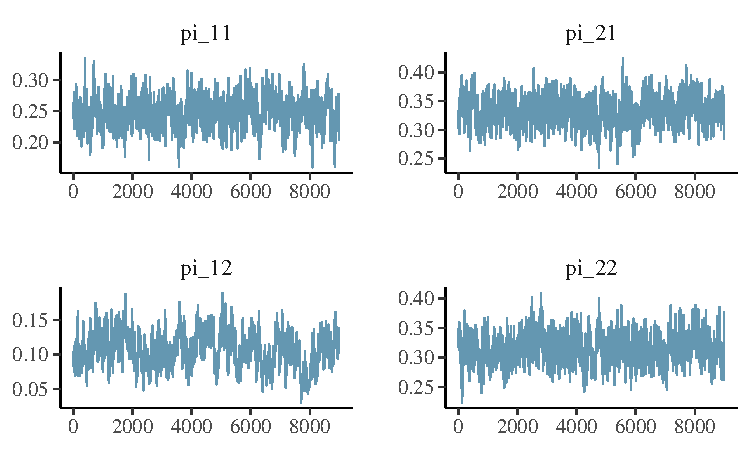
\includegraphics{dppaper_files/figure-latex/trace-plot-1} 

}

\caption{(Example 1) trace plots.}\label{fig:trace-plot}
\end{figure}

To see if there is evidence of gender bias we can look at the odds ratio.
Specifically, we look at the odds of a male being admitted to
that of female. A higher odds ratio would indicate a bias
favoring males. Figure \ref{fig:post-or-density} shows the posterior draws
from the dapper model. The large odds ratio values would seem
to indicate there is bias favoring the males. See (Bickel, Hammel, and O'Connell 1975) for
an explanation of the ``paradox'' of this result.

\begin{figure}

{\centering 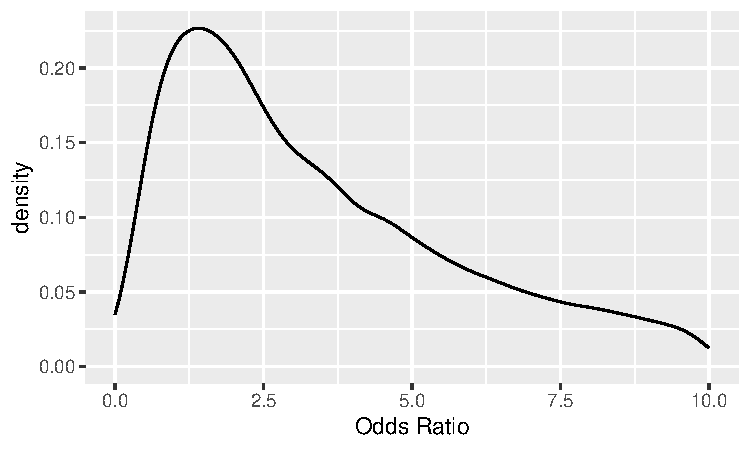
\includegraphics{dppaper_files/figure-latex/post-or-density-1} 

}

\caption{(Example 1) posterior density estimate for the odds ratio using 16,000 MCMC draws.}\label{fig:post-or-density}
\end{figure}

For comparison, we run a standard Bayesian analysis on the
noise infused table ignoring the privacy mechanism. This will
correspond exactly to the model defined in the \texttt{post\_f} component.
Figure \ref{fig:post-or-compare} shows a density estimate for the odds ratio
under the confidential and noisy data. The posterior
distribution for the odds ratio under the noisy data
is shifted significantly, indicating a large degree of bias.
Looking at left hand plot in figure \ref{fig:post-or-compare} shows the MAP estimate from \texttt{dapper}
is similar to that in the case of the confidential data.
The width of the posterior is also much larger since
it properly accounts for the uncertainty due to the privacy mechanism. This
illustrates the dangers of ignoring the privacy mechanism: a naive
analysis not only has bias, but also severely underestimates the
uncertainty associated with the odds ratio estimate.

\begin{figure}

{\centering 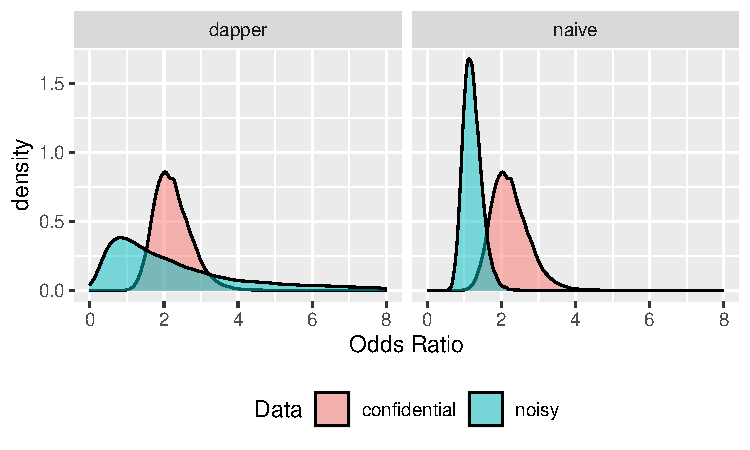
\includegraphics{dppaper_files/figure-latex/post-or-compare-1} 

}

\caption{(Example 1) comparison between using dapper and a naive Bayesian anaylsis on the
noise infused data and the original confidential data.}\label{fig:post-or-compare}
\end{figure}

\hypertarget{example-2-2x2-contingency-table-discrete-gaussian}{%
\subsection{Example 2: 2x2 Contingency Table (Discrete Gaussian)}\label{example-2-2x2-contingency-table-discrete-gaussian}}

To highlight the flexibility of \texttt{dapper} we reanalyze example 1
with a different privacy mechanism. For this example we taking inspiration from the US Census,
which is currently in the process of arguably the largest deployment of differential privacy.
Deploying large privacy system requires the careful analysis
of the privacy / utility trade-off of different candidate mechanisms. This is especially
true in the case of census data which has many users with different inference goals.
One of the mechanisms under consideration is the discrete Gaussian distribution.
In the context of the admissions data, this privacy mechanism works by injecting
noise into the the total cell counts given the 2x2 table. This is quite different from
example 1 where the randomized response scheme injected noise at the record level.
In fact, the discrete Gaussian distribution satisfies a privacy framework called
concentrated differential privacy (Canonne, Kamath, and Steinke 2021).
The strength of \texttt{dapper} comes from the fact we can analyze both scenarios under the
same framework.

Suppose we want to compare how our analysis from example 1 would look like
under the Census's discrete Gaussian privacy mechanism. Under the Census's
current privacy
parameters\footnote{There is only a direct relationship between zCDP and \((\epsilon, \delta)\)-differential privacy. To make comparisons between pure \(\epsilon\)-differential privacy and zCDP, the Census uses the value \(\delta = 10^{-10}\).}, setting
the scale parameter \(\sigma = 6.25\) implies a pure \(\epsilon\)-differential
privacy budget of \(2\log(3)\)\footnote{Canonne, Kamath, and Steinke (2021) showed \(\dfrac{1}{2} \epsilon^2\)-concentrated differential privacy implies \(\left(\dfrac{1}{2}\epsilon^2 + \epsilon \sqrt{2\log(1/\delta)}, \delta\right)\)-differential privacy.}. Using the \texttt{rdnorm} function allows
us to easily construct a hypothetical table privated using a discrete
Gaussian mechanism. {[}Label tables{]}

\begin{table}[!h]
\centering\caption{\label{tab:unnamed-chunk-14}Left table represents a random sub-sample of 400
    observations from the UCBAdmissions data set. The table on the right reprents
    the left table with independent discrete Gaussian noise added to each cell.}
\begin{table}

\centering
\begin{tabular}[t]{lrr}
\toprule
  & Admitted & Rejected\\
\midrule
Female & 46 & 118\\
Male & 109 & 127\\
\bottomrule
\end{tabular}
\end{table}\begin{table}

\centering
\begin{tabular}[t]{lrr}
\toprule
  & Admitted & Rejected\\
\midrule
Female & 47 & 110\\
Male & 110 & 131\\
\bottomrule
\end{tabular}
\end{table}
\end{table}

The US Census only releases cell counts, so a natural
statistic to consider is the vector of cell counts. As in
example 1, we imagine the latent database as a
\(400 \times 2\) binary matrix. Below
we describe the process for analyzing the privatized
data using \texttt{dapper}. Since the latent process
and posterior are the same as example 1, we only describe
how to construct \texttt{st\_f} and \texttt{priv\_f}. {[}MENTION TOTAL COUNTS ARE ALSO GIVEN{]}

\begin{enumerate}
\def\labelenumi{\arabic{enumi}.}
\item
  \texttt{st\_f}: The private summary statistic \(s_{dp}\) can be written as a record additive
  statistic using the indicator vectors \((1,0,0,0), (0,1,0,0), (0,0,0,1)\) and \((0,0,0,1)\).
  These four vectors correspond to the four possible cells.

\begin{verbatim}
st_f <- function(i, xi, sdp) {
  if(xi[1] & xi[2]) {
    c(1,0,0,0)
  } else if (xi[1] & !xi[2]) {
    c(0,1,0,0)
  } else if (!xi[1] & xi[2]) {
    c(0,0,1,0)
  } else {
    c(0,0,0,1)
  }
}
\end{verbatim}
\item
  \texttt{priv\_f}: The privacy mechanism us a discrete Gaussian distribution centered
  at 0.

\begin{verbatim}
priv_f <- function(sdp, tx) {
  sum(dapper::ddnorm(sdp - tx, mu = 0, sigma = 6.25, log = TRUE))
}
\end{verbatim}
\end{enumerate}

The summary table below show the results of running a chain for 2000 iterations with a burn-in of 1000 runs.

\begin{verbatim}
summary(dp_out)
\end{verbatim}

\begin{verbatim}
#> # A tibble: 4 x 10
#>   variable  mean median     sd    mad     q5   q95  rhat ess_bulk ess_tail
#>   <chr>    <dbl>  <dbl>  <dbl>  <dbl>  <dbl> <dbl> <dbl>    <dbl>    <dbl>
#> 1 pi_11    0.314  0.314 0.0278 0.0271 0.269  0.362  1.00     619.     874.
#> 2 pi_21    0.286  0.285 0.0264 0.0259 0.246  0.332  1.00     663.     762.
#> 3 pi_12    0.107  0.107 0.0209 0.0216 0.0743 0.143  1.00     355.     510.
#> 4 pi_22    0.293  0.293 0.0271 0.0281 0.249  0.337  1.00     508.     714.
\end{verbatim}

The posterior density estimate for the odds ratio is.

\begin{figure}

{\centering 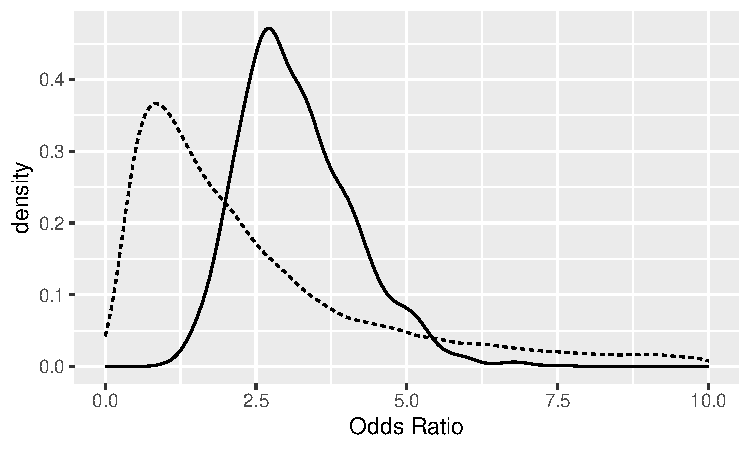
\includegraphics{dppaper_files/figure-latex/post-or-density-dg-1} 

}

\caption{(Example 2) posterior density estimate for the odds ratio using 1,000 MCMC draws.}\label{fig:post-or-density-dg}
\end{figure}

Like example 1, we can compare the naive analysis with the one under
the discrete Guassian mechanism. {[}FIX GRAPHS!{]}

\begin{figure}

{\centering 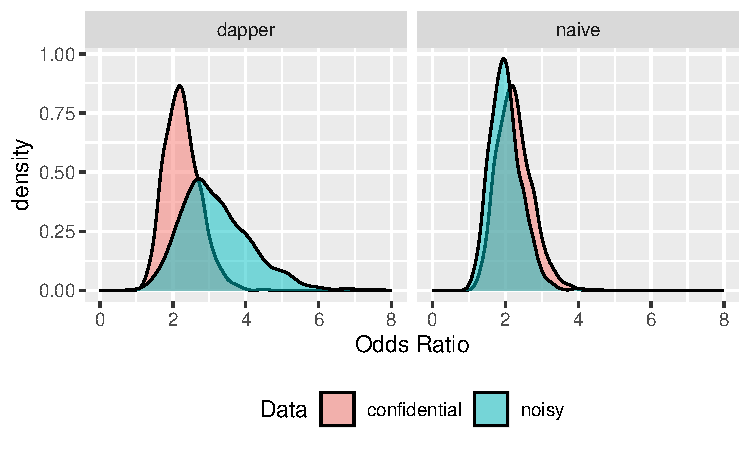
\includegraphics{dppaper_files/figure-latex/post-or-compare-dg-1} 

}

\caption{(Example 2) comparison between using dapper and a naive Bayesian anaylsis on the
noise infused data and the original confidential data.}\label{fig:post-or-compare-dg}
\end{figure}

\hypertarget{example-3-linear-regression}{%
\subsection{Example 3: Linear Regression}\label{example-3-linear-regression}}

In this section we apply \texttt{dapper} to reconstruct an
example presented in Ju et al. (2022). They apply a Laplace privacy
mechanism to a sufficient summary statistic for a linear regression model.
Let \(\{(x_i,y_i)\}_{i=1}^{n}\) be the original, confidential data with \(x_i \in \mathbb{R}^2\).
They assume the true data generating process follows the model

\[
\begin{aligned}
y &= -1.79 -2.89x_1 -0.66x_2 + \epsilon\\
\epsilon &\sim N(0,2^2)\\
\binom{x_1}{x_2} &\sim N_{2}(\mu, I_2)\\
\mu &= \binom{0.9}{-1.17}.
\end{aligned}
\]

Note, in most settings involving linear regression, the covariates are assumed to be
fixed, known constants. Thus the formulation above is a departure from the norm since
we are assuming a random design matrix. More details on why this framing is necessary
will be provided later when describing the latent model.

The paper considers the scenario where one desires to publicly release the
sufficient summary statistics

\[
s(x,y) = (x^Ty, y^Ty, x^Tx).
\]

This summary statistic satisfies the additive record property since \(s(x,y) = \sum_{i=1}^{n} t(x_i, y_i)\)
where

\[
t(x_i,y_i) = ((x_{i})^T y_i, y_i^2, (x_{i})^T x_i),
\]

with \(\epsilon\)-DP privacy guarantees. To achieve this guarantee it is
necessary to bound the value of the statistic. This will ensure
a data point cannot be too ``unique.'' Intuitively, an outlier is
easy to identify, so we want to make sure no data point
is an extreme outlier. In the language of differential
privacy, this equates to bounding the global sensitivity. This was accomplished
by clamping the data. More precisely, we define
the clamp function \([z] := \min\{\max\{z,-10\}, 10\}\) which truncates a value
\(z\) so that it falls into the interval \([-10,10]\). Furthermore, we let \(\tilde{z} := [z]/10\)
denote the normalized clamped value of \(z\). The clamped statistic is

\[
t(x_i,y_i) = ((\tilde{x}^{i})^T \tilde{y}_i, \tilde{y}_i^2, (\tilde{x}_{i})^T \tilde{x}_i).
\]

Ignoring duplicate entries, the global sensitivity is \(\Delta = p^2 + 4p + 3\) \footnote{The original paper, Ju et al. (2022), contains a computation error and uses \(\Delta = p^2 + 3p + 3\)}.
Using the Laplace mechanism, \(\epsilon\)-DP privacy can thus be achieved by adding i.i.d. Laplace\((0, \Delta/\epsilon)\)
error to each unique entry. A tighter bound on sensitivity can be achieved using
other techniques, see (Awan and Slavković 2020).

\begin{enumerate}
\def\labelenumi{\arabic{enumi}.}
\item
  \texttt{latent\_f}: Since the privacy mechanism involves injecting noise into the design
  matrix, it is not possible to use the standard approach where one assumes the design
  matrix is a fixed, known constant. Hence to draw a sample from the latent data generating
  process we use the relation \(f(x,y) = f(x)f(y \mid x)\). In this formulation,
  it is necessary to specify a distribution on the covariates \(x\).

\begin{verbatim}
latent_f <- function(theta) {
  xmat <- MASS::mvrnorm(50 , mu = c(.9,-1.17), Sigma = diag(2))
  y <- cbind(1,xmat) %*% theta + rnorm(50, sd = sqrt(2))
  cbind(y,xmat)
}
\end{verbatim}
\item
  \texttt{post\_f}: Given confidential data \(X\) we can derive the posterior analytically
  using a normal prior on \(\beta\).
  \[
  \begin{aligned}
  \beta &\sim N_{p+1}(0, \tau^2 I_{p+1})\\
  \beta \mid x,y &\sim N(\mu_n, \Sigma_n)\\
  \Sigma_n &= (x^Tx/\sigma^2 + I_{p+1}/\tau^2)^{-1}\\
  \mu_n &= \Sigma_n(x^Ty)/\sigma^2
  \end{aligned}
  \]
  In the example, we use \(\sigma^2 = 2\) and \(\tau^2 = 4\).

\begin{verbatim}
post_f <- function(dmat, theta) {
  x <- cbind(1,dmat[,-1])
  y <- dmat[,1]

  ps_s2 <- solve((1/2) * t(x) %*% x + (1/4) * diag(3))
  ps_m <- ps_s2 %*% (t(x) %*% y) * (1/2)

  MASS::mvrnorm(1, mu = ps_m, Sigma = ps_s2)
}
\end{verbatim}
\item
  \texttt{st\_f}: The summary statistic contains duplicate
  entries. We can considerable reduce the dimension of the
  statistic by only considering unique entries. The \texttt{clamp\_data}
  function is used to bound the statistic to give a finite
  global sensitivity.

\begin{verbatim}
clamp_data <- function(dmat) {
  pmin(pmax(dmat,-10),10) / 10
}

st_f <- function(i, tx, sdp) {
  txc <- clamp_data(tx)
  ydp <- txc[1]
  xdp <- cbind(1,t(txc[-1]))

  s1 <- t(xdp) %*% ydp
  s2 <- t(ydp) %*% ydp
  s3 <- t(xdp) %*% xdp

  ur_s1 <- c(s1)
  ur_s2 <- c(s2)
  ur_s3 <- s3[upper.tri(s3,diag = TRUE)][-1]
  c(ur_s1,ur_s2,ur_s3)
}
\end{verbatim}
\item
  \texttt{priv\_f}: Privacy Mechanism
  adds Laplace\((0, \Delta/\epsilon)\) error to each unique entry
  of the statistic. In this example, \(\Delta = 15\) and \(\epsilon = 10\).

\begin{verbatim}
priv_f <- function(sdp, zt) {
  sum(VGAM::dlaplace(sdp - zt, 0, 15/10, log = TRUE))
}
\end{verbatim}
\end{enumerate}

First we simulate fake data using the aforementioned privacy mechanism.
In the example, we use \(n = 50\) observations.

\begin{verbatim}
deltaa <- 15
epsilon <- 10
n <- 50

set.seed(1)
xmat <- MASS::mvrnorm(n, mu = c(.9,-1.17), Sigma = diag(2))
beta <- c(-1.79, -2.89, -0.66)
y <- cbind(1,xmat) %*% beta + rnorm(n, sd = sqrt(2))

#clamp the confidential data in xmat
dmat <- cbind(y,xmat)
sdp <-  apply(sapply(1:nrow(dmat), function(i) st_f(i, dmat[i,], sdp)), 1, sum)

#add Laplace noise 
sdp <- sdp + VGAM::rlaplace(length(sdp), location = 0, scale = deltaa/epsilon)
\end{verbatim}

We construct a privacy model using the \texttt{new\_privacy} function and
make 25,000 MCMC draws with a burn in of 1000 draws.

\begin{verbatim}
library(dapper)

dmod <- new_privacy(post_f   = post_f,
                    latent_f = latent_f,
                    priv_f   = priv_f,
                    st_f     = st_f,
                    npar     = 3,
                    varnames = c("beta0", "beta1", "beta2"))



dp_out <- dapper_sample(dmod,
                        sdp = sdp,
                        niter = 25000,
                        warmup = 1000,
                        chains = 1,
                        init_par = rep(0,3))
\end{verbatim}

The output of the MCM run is reported below.

\begin{verbatim}
summary(dp_out)
\end{verbatim}

\begin{verbatim}
#> # A tibble: 3 x 10
#>   variable   mean median    sd   mad    q5   q95  rhat ess_bulk ess_tail
#>   <chr>     <dbl>  <dbl> <dbl> <dbl> <dbl> <dbl> <dbl>    <dbl>    <dbl>
#> 1 beta0    -0.900 -0.821  1.49  1.47 -3.49 1.41   1.00     471.    1082.
#> 2 beta1    -2.22  -2.42   1.22  1.03 -3.91 0.136  1.00     231.     329.
#> 3 beta2     0.511  0.454  1.28  1.36 -1.48 2.70   1.00     224.     480.
\end{verbatim}

For comparison, we consider a Bayesian analysis where the design matrix
is a fixed known constant and \(\sigma^2\) is known. Using the
diffuse prior \(f(\beta) \propto 1\) leads to normal posterior.
\[
\begin{aligned}
f(\beta \mid x,y, \sigma^2) &\sim N(\hat{\beta}, \hat{\Sigma})\\
\hat{\mu} &= (x^Tx)^{-1}xy\\
\hat{\Sigma} &= \sigma^{2}(x^Tx)^{-1}
\end{aligned}
\]

The posterior can be written as a function of \(s(x,y)\). Since
we only have access to the noisy version \(s_{dp}\) we can
attempt to reconstruct the posterior be extracting the
relevant entries which is done below.

Because of the injected privacy noise, the reconstructed
\((x^Tx)^{-1}\) matrix is not positive definite. As
a naive solution we use the algorithm proposed\\
in (Higham 1988) to find the closest positive semi-definite matrix
as determined by the Forbenius norm. The \texttt{pracma}
package contains an implementation via the \texttt{nearest\_psd}
function.

Figure \ref{fig:regression-compare} shows the posterior density estimates for the \(\beta\) coefficients based
on \(s_{dp}\). The density estimates indicates the naive method, which ignores the privacy mechanism, has bias and
underestimates the variance. Likewise Figure \ref{fig:regression-data-compare}
illustrates how dapper provides point estimates that are not far off from those
that would have been obtained using the original confidential data. And the dramatic
increase in the posterior variance indicates the privacy mechanism adds substantial
uncertainty to the estimates.

\begin{figure}

{\centering 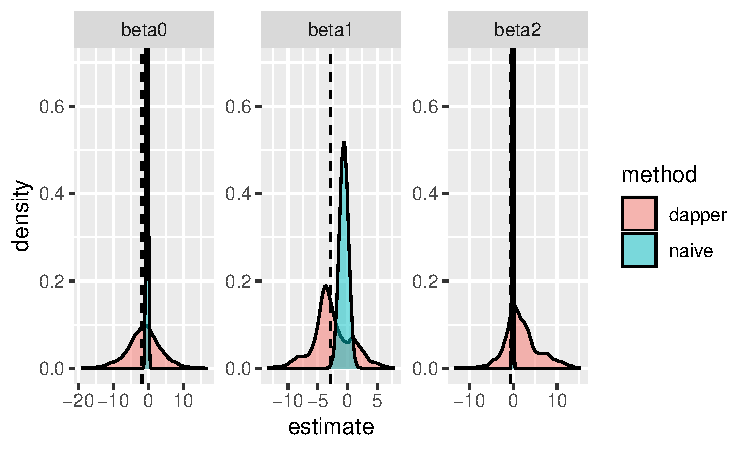
\includegraphics{dppaper_files/figure-latex/regression-compare-1} 

}

\caption{(Example 3) comparison between dapper and a naive approach that ignores the privacy mechanism. 
The dashed lines are the true coefficient values.}\label{fig:regression-compare}
\end{figure}

\begin{figure}

{\centering 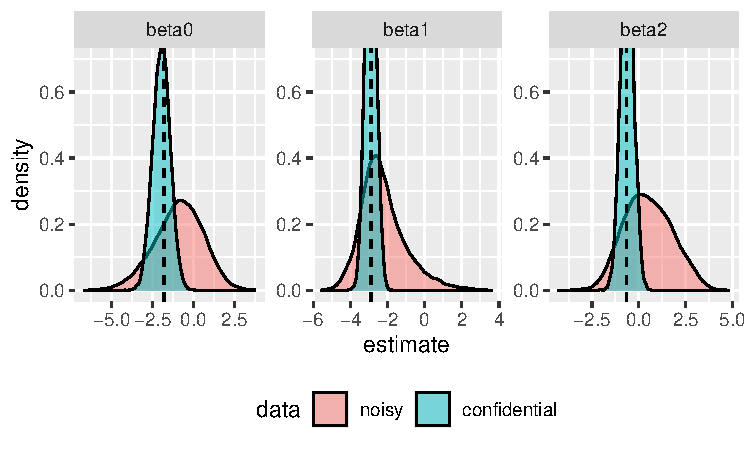
\includegraphics{dppaper_files/figure-latex/regression-data-compare-1} 

}

\caption{(Example 3) comparison for example between using dapper on the noisy data set and a standard
Bayesian analysis on the confidential data set.}\label{fig:regression-data-compare}
\end{figure}

\hypertarget{discussion}{%
\section{Discussion}\label{discussion}}

\hypertarget{mixing-and-privacy-loss-budget}{%
\subsection{Mixing and Privacy Loss Budget}\label{mixing-and-privacy-loss-budget}}

Mixing can be poor when the posterior under a given privacy mechanism is
much wider than the posterior that would arise using the confidential data. In
other words, when the privacy budget is small, poor mixing can be expected. Intuitively,
this issue arises because the step size of the chain is governed by the variance
of the posterior model (step 1 of the algorithm) that assumes no privacy noise. Thus, a small privacy budget
will generate a chain whose step sizes are too small to effectively explore the
private posterior.The rest of this section explores a toy example that will provide insight into this
phenomenon.

Suppose the confidential data consist of a single observation \(x \in \mathbb{R}\),
and consider the scenario where a user makes a request to view \(x\) and
in return receives \(s := x + \nu\), which is a noise infused version of \(x\).
For simplicity, we do not worry about constructing an \(\epsilon\)-DP privacy mechanism,
and take \(\nu \sim N(0, \epsilon^{-2})\) for some \(\epsilon > 0\). However, it
will still be useful to think of \(\epsilon\) as the privacy budget since smaller values
of \(\epsilon\) correspond to a larger amounts of noise. Using
a flat prior and a normally distributed likelihood results in
a normally distributed posterior described below.

\[
\begin{aligned}
f(\theta) &\propto 1\\
s \mid x &\sim N(x, \epsilon^{-2})\\
x \mid \theta &\sim N(\theta, \sigma^2)\\
\end{aligned}
\]

With the above model, the data augmentation process consist of the
two steps

\begin{itemize}
\item
  Step 1: Sample from \(x \mid \theta, s \sim N(\mu, \tau^2)\), where
  \(\mu\) and \(\tau\) are defined as:
  \[
  \begin{aligned}
  \mu &:= \dfrac{\dfrac{1}{\epsilon^{-2}}s + \dfrac{1}{\sigma^2}\theta}{\dfrac{1}{\epsilon^{-2}} + \dfrac{1}{\sigma^2}}\\
  \tau^2 &:= \dfrac{1}{\dfrac{1}{\epsilon^{-2}} + \dfrac{1}{\sigma^2}}.
  \end{aligned}
  \]
\item
  Step 2: Sample from \(\theta \mid x, s \sim N(x, \sigma^2)\).
\end{itemize}

In the setting of this example, (Liu and Wu 1999) showed the Bayesian fraction of missing information
gives the exact convergence rate. The Bayesian fraction of missing information, \(\gamma\) is
defined as
\begin{align*}
\gamma &:= 1 - \dfrac{E[Var(\theta \mid s, x) \mid s]}{Var(\theta \mid s)} = 1 - \dfrac{E[Var(\theta \mid x)]}{Var(\theta \mid s)}.
\end{align*}

Plugging in the appropriate quantities into the above panel gives us

\begin{align*}
\gamma &= 1 - \dfrac{\sigma^2}{\sigma^2 + \epsilon^{-2}} = 1 - \dfrac{1}{1 + \dfrac{\epsilon^{-2}}{\sigma^2}}.
\end{align*}

The chain converges faster as \(\gamma \to 0\) an slower as \(\gamma \to 1\).
From the right hand term in the above panel, we can see \(\gamma\)
depends only on \(\epsilon^{-2}/\sigma^2\) and as the privacy budget decreases (i.e.~more noise is being added to \(x\)),
\(\gamma \to 1\).

Thus when poor mixing is observed, we recommend seeing if increasing the privacy
budget helps. Unfortunately, if one is not at liberty to alter the privacy budget,
there is no quick fix, and other sampling scheme may be needed.
In the case where a small privacy budget results
in a posterior much more diffuse than under the confidential data set, one
can draw samples using the pseudo-likelihood scheme as proposed in (Andrieu and Roberts 2009). This
scheme fits in the same data augmentation framework as \texttt{dapper} but is not implemented.

\hypertarget{related-work}{%
\subsection{Related Work}\label{related-work}}

Adjusting statistical workflows to account for added noise in covariates
is extensively studied in the context of measurement error (e.g.~noisy sensor readings)
and there exists readily available tools for making the proper adjustments.
For textbook length treatments on the topic see (Yi 2017; Carroll et al. 2006).
Work in this area mostly focuses on methods which do not require fully specifying the
measurement error model, since this is often assumed unknown.
However, in differential privacy, the measurement error model is exactly known.
This difference, makes feasible some ideas which the measurement
error community has not previously considered (Smith 2011; Karwa, Kifer, and Slavković 2015b).

\hypertarget{summary}{%
\section{Summary}\label{summary}}

Currently, there is a lack of software tools privacy researchers can use
to evaluate the impact of privacy mechanisms on statistical analyses.
While there have been tremendous gains in the theoretical aspects of privacy,
the lack of software resources to deploy and work with new privacy techniques has
hampered their adoption. This gap in capability has been noted by several
large industry entities who have begun building software ecosystems for
working with differential privacy. SmartNoise by Microsoft {[}insert citation{]} and SafeTab {[}insert citation{]} by the US Census, for example,
are tools for generating synthetic data that has differentially private guarantees.
However, the majority of these software tools only address privacy and not the
ensuing analysis or, if it does, address the analysis only for specific models.
Privacy researchers currently lack good tools for evaluating the impact
of privacy mechanisms on a statistical analysis.

Thus \texttt{dapper} helps fill an urgent need by providing researchers a way to properly account
for the noise introduced for privacy protection in their statistical analysis. A notable
feature is its flexibility which allows the users to specify a custom
privacy mechanism. The benefit being that \texttt{dapper} can evaluate already
established privacy mechanisms and those that have yet to be discovered.

\texttt{dapper} offers a significant step forward in providing general-purpose statistical
inference tools for privatized data. Despite the strengths of \texttt{dapper}, there
are notable weaknesses, which highlight the important directions for future work.
Weaknesses include the requirement for the privacy mechanism to have a density
(e.g.~the exponential mechanism has no density). The non-private posterior needs
a relatively efficient sampler. Slow convergence when the privacy budget is small,
and a statistic that satisfies record additivity to fully leverage \texttt{dapper} computational
potential.

\hypertarget{references}{%
\section*{References}\label{references}}
\addcontentsline{toc}{section}{References}

\hypertarget{refs}{}
\begin{CSLReferences}{1}{0}
\leavevmode\vadjust pre{\hypertarget{ref-Abowd2018}{}}%
Abowd, John M. 2018. {``The u.s. Census Bureau Adopts Differential Privacy.''} In \emph{Proceedings of the 24th ACM SIGKDD International Conference on Knowledge Discovery \&Amp; Data Mining}. KDD '18. ACM. \url{https://doi.org/10.1145/3219819.3226070}.

\leavevmode\vadjust pre{\hypertarget{ref-Andrieu2009}{}}%
Andrieu, Christophe, and Gareth O. Roberts. 2009. {``The Pseudo-Marginal Approach for Efficient Monte Carlo Computations.''} \emph{The Annals of Statistics} 37 (2). \url{https://doi.org/10.1214/07-aos574}.

\leavevmode\vadjust pre{\hypertarget{ref-Awan2020}{}}%
Awan, Jordan, and Aleksandra Slavković. 2020. {``Structure and Sensitivity in Differential Privacy: Comparing k-Norm Mechanisms.''} \emph{Journal of the American Statistical Association} 116 (534): 935--54. \url{https://doi.org/10.1080/01621459.2020.1773831}.

\leavevmode\vadjust pre{\hypertarget{ref-Bickel1975}{}}%
Bickel, Peter J., Eugene A. Hammel, and John W. O'Connell. 1975. {``Sex Bias in Graduate Admissions: Data from Berkeley: Measuring Bias Is Harder Than Is Usually Assumed, and the Evidence Is Sometimes Contrary to Expectation.''} \emph{Science} 187 (4175): 398--404. \url{https://doi.org/10.1126/science.187.4175.398}.

\leavevmode\vadjust pre{\hypertarget{ref-Canonne2021}{}}%
Canonne, Clément L., Gautam Kamath, and Thomas Steinke. 2021. {``The Discrete Gaussian for Differential Privacy.''} \url{https://arxiv.org/abs/2004.00010}.

\leavevmode\vadjust pre{\hypertarget{ref-Carroll2006}{}}%
Carroll, Raymond J., David Ruppert, Leonard A. Stefanski, and Ciprian M. Crainiceanu. 2006. \emph{Measurement Error in Nonlinear Models}. Chapman; Hall/CRC. \url{https://doi.org/10.1201/9781420010138}.

\leavevmode\vadjust pre{\hypertarget{ref-ding2017collecting}{}}%
Ding, Bolin, Janardhan Kulkarni, and Sergey Yekhanin. 2017. {``Collecting Telemetry Data Privately.''} \url{https://arxiv.org/abs/1712.01524}.

\leavevmode\vadjust pre{\hypertarget{ref-Dwork2006}{}}%
Dwork, Cynthia, Frank McSherry, Kobbi Nissim, and Adam Smith. 2006. {``Calibrating Noise to Sensitivity in Private Data Analysis.''} In \emph{Lecture Notes in Computer Science}, 265--84. Springer Berlin Heidelberg. \url{https://doi.org/10.1007/11681878_14}.

\leavevmode\vadjust pre{\hypertarget{ref-Erlingsson_2014}{}}%
Erlingsson, Úlfar, Vasyl Pihur, and Aleksandra Korolova. 2014. {``RAPPOR: Randomized Aggregatable Privacy-Preserving Ordinal Response.''} In \emph{Proceedings of the 2014 ACM SIGSAC Conference on Computer and Communications Security}. CCS'14. ACM. \url{https://doi.org/10.1145/2660267.2660348}.

\leavevmode\vadjust pre{\hypertarget{ref-Gong2022}{}}%
Gong, Ruobin. 2022. {``Transparent Privacy Is Principled Privacy.''} \emph{Harvard Data Science Review}, no. Special Issue 2 (June). \url{https://doi.org/10.1162/99608f92.b5d3faaa}.

\leavevmode\vadjust pre{\hypertarget{ref-Higham1988}{}}%
Higham, Nicholas J. 1988. {``Computing a Nearest Symmetric Positive Semidefinite Matrix.''} \emph{Linear Algebra and Its Applications} 103 (May): 103--18. \url{https://doi.org/10.1016/0024-3795(88)90223-6}.

\leavevmode\vadjust pre{\hypertarget{ref-Ju2022}{}}%
Ju, Nianqiao, Jordan Awan, Ruobin Gong, and Vinayak Rao. 2022. {``Data Augmentation {MCMC} for Bayesian Inference from Privatized Data.''} In \emph{Advances in Neural Information Processing Systems}, edited by Alice H. Oh, Alekh Agarwal, Danielle Belgrave, and Kyunghyun Cho. \url{https://openreview.net/forum?id=tTWCQrgjuM}.

\leavevmode\vadjust pre{\hypertarget{ref-Karwa2015}{}}%
Karwa, Vishesh, Dan Kifer, and Aleksandra B. Slavković. 2015b. {``Private Posterior Distributions from Variational Approximations.''} \url{https://arxiv.org/abs/1511.07896}.

\leavevmode\vadjust pre{\hypertarget{ref-karwa2015private}{}}%
---------. 2015a. {``Private Posterior Distributions from Variational Approximations.''} \url{https://arxiv.org/abs/1511.07896}.

\leavevmode\vadjust pre{\hypertarget{ref-Kenny2021}{}}%
Kenny, Christopher T., Shiro Kuriwaki, Cory McCartan, Evan T. R. Rosenman, Tyler Simko, and Kosuke Imai. 2021. {``The Use of Differential Privacy for Census Data and Its Impact on Redistricting: The Case of the 2020 u.s. Census.''} \emph{Science Advances} 7 (41). \url{https://doi.org/10.1126/sciadv.abk3283}.

\leavevmode\vadjust pre{\hypertarget{ref-Liu1999}{}}%
Liu, Jun S., and Ying Nian Wu. 1999. {``Parameter Expansion for Data Augmentation.''} \emph{Journal of the American Statistical Association} 94 (448): 1264--74. \url{https://doi.org/10.1080/01621459.1999.10473879}.

\leavevmode\vadjust pre{\hypertarget{ref-Robert2004}{}}%
Robert, Christian P., and George Casella. 2004. \emph{Monte Carlo Statistical Methods}. \emph{Springer Texts in Statistics}. Springer New York. \url{https://doi.org/10.1007/978-1-4757-4145-2}.

\leavevmode\vadjust pre{\hypertarget{ref-SantosLozada2020}{}}%
Santos-Lozada, Alexis R., Jeffrey T. Howard, and Ashton M. Verdery. 2020. {``How Differential Privacy Will Affect Our Understanding of Health Disparities in the United States.''} \emph{Proceedings of the National Academy of Sciences} 117 (24): 13405--12. \url{https://doi.org/10.1073/pnas.2003714117}.

\leavevmode\vadjust pre{\hypertarget{ref-Smith2011}{}}%
Smith, Adam. 2011. {``Privacy-Preserving Statistical Estimation with Optimal Convergence Rates.''} In \emph{Proceedings of the Forty-Third Annual ACM Symposium on Theory of Computing}. STOC'11. ACM. \url{https://doi.org/10.1145/1993636.1993743}.

\leavevmode\vadjust pre{\hypertarget{ref-tang2017privacy}{}}%
Tang, Jun, Aleksandra Korolova, Xiaolong Bai, Xueqiang Wang, and Xiaofeng Wang. 2017. {``Privacy Loss in Apple's Implementation of Differential Privacy on MacOS 10.12.''} \url{https://arxiv.org/abs/1709.02753}.

\leavevmode\vadjust pre{\hypertarget{ref-Wang2018}{}}%
Wang, Yue, Daniel Kifer, Jaewoo Lee, and Vishesh Karwa. 2018. {``Statistical Approximating Distributions Under Differential Privacy.''} \emph{Journal of Privacy and Confidentiality} 8 (1). \url{https://doi.org/10.29012/jpc.666}.

\leavevmode\vadjust pre{\hypertarget{ref-NIPS2010_sherry}{}}%
Williams, Oliver, and Frank Mcsherry. 2010. {``Probabilistic Inference and Differential Privacy.''} In \emph{Advances in Neural Information Processing Systems}, edited by J. Lafferty, C. Williams, J. Shawe-Taylor, R. Zemel, and A. Culotta. Vol. 23. Curran Associates, Inc. \url{https://proceedings.neurips.cc/paper_files/paper/2010/file/fb60d411a5c5b72b2e7d3527cfc84fd0-Paper.pdf}.

\leavevmode\vadjust pre{\hypertarget{ref-Winkler2021}{}}%
Winkler, Richelle L., Jaclyn L. Butler, Katherine J. Curtis, and David Egan-Robertson. 2021. {``Differential Privacy and the Accuracy of County-Level Net Migration Estimates.''} \emph{Population Research and Policy Review} 41 (2): 417--35. \url{https://doi.org/10.1007/s11113-021-09664-5}.

\leavevmode\vadjust pre{\hypertarget{ref-Yi2017}{}}%
Yi, Grace Y. 2017. \emph{Statistical Analysis with Measurement Error or Misclassification}. \emph{Springer Series in Statistics}. Springer New York. \url{https://doi.org/10.1007/978-1-4939-6640-0}.

\end{CSLReferences}


\address{%
Kevin Eng\\
Rutgers University\\%
Department of Statistics\\ Piscataway, NJ 08854\\
%
\url{https://www.britannica.com/animal/quokka}\\%
%
\href{mailto:ke157@stat.rutgers.edu}{\nolinkurl{ke157@stat.rutgers.edu}}%
}

\address{%
Jordan A. Awan\\
Purdue University\\%
Department of Statistics\\ West Lafayette, IN 47907\\
%
\url{https://jordan-awan.com/}\\%
%
\href{mailto:jawan@purdue.edu}{\nolinkurl{jawan@purdue.edu}}%
}

\address{%
Ruobin Gong\\
Rutgers University\\%
Department of Statistics\\ Piscataway, NJ 08854\\
%
\url{https://ruobingong.github.io/}\\%
%
\href{mailto:ruobin.gong@rutgers.edu}{\nolinkurl{ruobin.gong@rutgers.edu}}%
}

\address{%
Nianqiao Phyllis Ju\\
Purdue University\\%
Department of Statistics\\ West Lafayette, IN 47907\\
%
\url{https://nianqiaoju.github.io/}\\%
%
\href{mailto:nianqiao@purdue.edu}{\nolinkurl{nianqiao@purdue.edu}}%
}

\address{%
Vinayak A. Rao\\
Purdue University\\%
Department of Statistics\\ West Lafayette, IN 47907\\
%
\url{https://varao.github.io/}\\%
%
\href{mailto:varao@purdue.edu}{\nolinkurl{varao@purdue.edu}}%
}
